
\chapter{Interface homme machine}
\minitoc

\section{Fonctionnalités de l' IHM}

L'interface homme-machine est une des composantes essentielles de notre projet.
En effet, c'est en grande partie grâce à elle que l'utilisateur va pouvoir juger de la qualité du logiciel.
Ainsi, conformément au cahier des charges, on va retrouver les fonctionnalités suivantes~:

\begin{enumerate}

\item Editeur de texte~: Editeur conçu pour que l'utilisateur réalise des prises de notes.
L'éditeur est composé des éléments suivants~:
\begin{itemize}
\item Outils de formatage,
\item Affichage du plan.
\end{itemize}
\item Visualisation du cours~: Panneau pour visualiser le cours prononcé par l'enseignant, en provenance du moteur de reconnaissance vocale.
\item Explorateur de documents~: Possibilité pour l'utilisateur de parcourir ses cours et de les organiser.
On y retrouve les trois éléments suivants~:
\begin{itemize}
\item Module,
\item Dossier,
\item Cours.
\end{itemize}
\item Outils d'import et d'export~: Pour permettre à l'utilisateur d'utiliser ses supports de cours sur différentes plateformes ou encore de les imprimer, les fonctionnalités suivantes sont disponibles~:
\begin{itemize}
\item Export au format PDF,
\item Export/import au format RTF (Format Microsoft, compatible Word),
\item Impression du cours édité.
\end{itemize} 
\item Outils de configuration du moteur de reconnaissance vocale.  
\end{enumerate}

L'ensemble de ces fonctionnalités n'était pas figé lors du processus de développement, elles ont donc été ajoutées au fur et à mesure des cycles de celui-ci.

\section{Ergonomie}

\subsection{Solutions de visualisation et d'édition envisagées}

\subsubsection{Solution 1}

En ce qui concerne l'ergonomie du logiciel plusieurs choix de conception ont été mis en confrontation. Le premier, qui n'a finalement pas été retenu était d'utiliser un unique éditeur de texte. Celui-ci aurai joué un  double rôle, tout d'abord celui d'un panneau de visualisation du cours, prononcé par l'enseignant. Le cours aurai été affiché à la fin du document. De plus, l'utilisateur aurai eu la possibilité de modifier le panneau de visualisation dans le but d'organiser son  cours.

Le principal soucis de cette solution était que le travail de restructuration du cours en direct aurai été une tâche particulièrement fastidieuse et aurai fortement perturber la suivie du cours.


\subsubsection{Solution 2}

La solution finalement envisagée est l'utilisation de deux panneaux. Un premier dont le but est d'afficher le texte brut, issu du moteur de reconnaissance vocale. Celui-ci  va permettre à l'utilisateur malentendant d'utiliser sa  vision en remplacement de son ouïe. Le second panneau sert quand à lui de support de cours, offrant notamment la possibilité de prise de notes. De la même façon qu'un étudiant normal prendrai des notes sur papier.

Bien que cette solution semble la plus productive et la plus intéressante, elle est n'est pas exempt de défauts. Ainsi, il faut bien souligner le fait qu'il est particulièrement difficile de lire un texte tout en réalisant des prises de notes. Ainsi, même si cette solution semble plus difficile pour les utilisateurs moins familiers avec l'informatique, elle constitue pour nous la meilleure solution pour répondre au besoin de saisie d'un cours.On notera également que pour un utilisateur familier avec l'informatique, le fait de saisir un texte sans regarder le clavier ne pose pas de problèmes particuliers, lui laissant ainsi la possibilité de lire facilement le texte issue du moteur de reconnaissance.


\subsection{Accessibilité}

Un des points fondamentaux de l'IHM était de concevoir une interface intuitive et facile d'utilisation. Ainsi, un effort particulier à été consacré a l'accessibilité de l'outil, de sorte que l'utilisateur prenne rapidement en main l'outil. Pour cela, différents points ont étés réalisés :

\begin{enumerate}
 \item Une barre d'outils avec des icônes explicites : pour permettre un accès rapide au principales fonctions
 \item Création de raccourcis claviers classiques (CTRL-C, CTRL-V ...)
 \item Utilisation des standards d'ergonomie : Placement des menus, des boutons ...
\end{enumerate}

\subsection{Tests ergonomiques}

En raison de problèmes de temps, il n'a malheureusement pas été possible de réaliser des tests d'ergonomie avec un étudiant mal-entendant. Cependant  l'approche idéale pour la réalisation de cette IHM, aurai été de suive un cycle de développement basé sur des méthodes agiles orientées vers l'utilisateur. Notamment l'utilisation de XP, de Scrum ou encore de la méthode LUCID\footnote{devernay.free.fr/cours/IHM/lucid.pdf}.


\section{Conception MVC}

En ce qui concerne la conception de l'application elle s'organise suivant le pattern MVC\footnote{J2EE Architecture Approaches : http://java.sun.com/} : Model View Controler. Le but d'une telle architecture est de bien diviser les différentes couches de l'application. On retrouve ainsi une couche Model, gérant les entités de la base de donnée (utilisation du pattern DAO); une couche View, à laquelle on associe l'interface graphique réalisée en swing; et enfin une couche intermédiaire controller, qui comme son nom l'indique sert à contrôler les deux autres couches via des mécanismes de synchronisation, notamment via l'utilisation du pattern Observer. 



\begin{figure}[h]
 \centering
 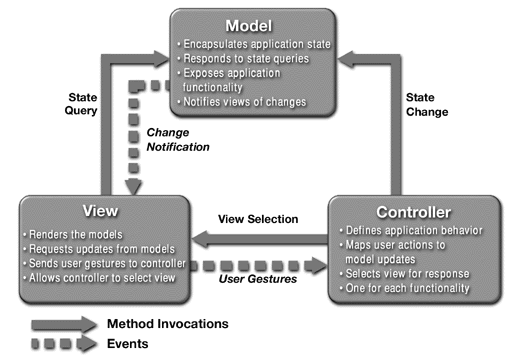
\includegraphics[scale=0.8]{./images/mvc.png}
 % homePanel.png: 0x0 pixel, -2147483648dpi, 0.00x0.00 cm, bb=
 \caption{IHM - Architecture MVC }
 \label{fig:mvc}
\end{figure}


Le diagramme \ref{fig:ihmUMLl} montre l'organisation des différentes classes de l'application. Comme on peut le voir, l'IHM est découpée suivant les principaux panels qui la compose. De plus, on distingue clairement la séparation entre les différentes couches de l'application. La classe Controller au centre, et le moteur de reconnaissance, qui ici fait office de couche Métier\footnote{Pour des raison de lisibilité, le module de gestion de la base de donnée n'est pas présent sur ce diagramme}.



\begin{figure}[h]
 \centering
 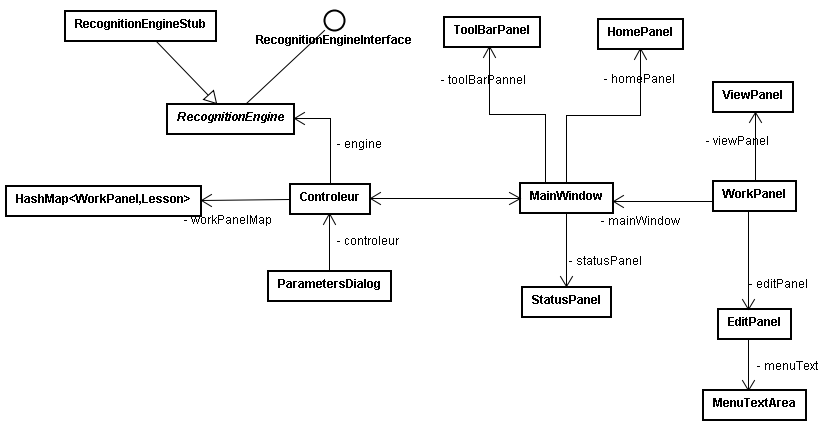
\includegraphics[scale=0.5]{./images/ihmUML.png}
 % homePanel.png: 0x0 pixel, -2147483648dpi, 0.00x0.00 cm, bb=
 \caption{IHM - Diagramme de classes}
 \label{fig:ihmUMLl}
\end{figure}


\section{Captures d'écran}

\subsection{Panneau d'accueil}


La figure \ref{fig:homePanel} montre le l'application au lancement de l'interface. Comme on peut le voir le panneau de gauche contient la liste des cours de l'utilisateur. Il peut ainsi les organiser facilement à la manière d'un explorateur de fichier classique. (Actions glisser déposer, création d'éléments ...). Sur la partie droite on retrouve la liste des documents de l'utilisateur. Cependant, pour des raisons d'ergonomie, ce panneau vise à offrir une organisation différente des cours. Il est ainsi possible de trier ses cours en fonction de leurs date de modification, de création ... Il faut noter que le changement de l'organisation sur ce panneau ne modifie pas l'organisation du panneau de gauche qui est indépendante.


\begin{figure}[H]
 \centering
 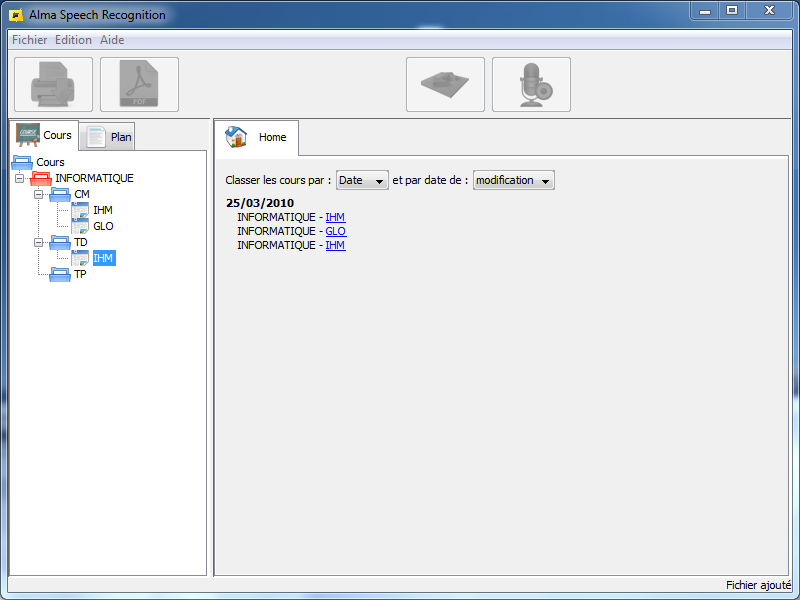
\includegraphics[scale=0.6]{./images/homePanel.png}
 % homePanel.png: 0x0 pixel, -2147483648dpi, 0.00x0.00 cm, bb=
 \caption{IHM - Panneau d'accueil}
 \label{fig:homePanel}
\end{figure}




\subsection{Panneau de travail}

La figure \ref{fig:workPanel} représente la même fenêtre que celle présente sur la figure \ref{fig:homePanel}. Cependant, ici on peut voir qu'un cours à été ouvert. L'ensemble des cours ouvert sont accessibles dans les différents onglets qui composent la fenêtre. Sur la figure \ref{fig:workPanel}, on remarque que les cours IMH et GLO sont ouverts simultanément.

Toujours sur cette fenêtre, on peut voir que chaque cours (onglet) se divise en deux parties : la partie visualisation du cours, qui affiche de façon continue la sortie du moteur de reconnaissance vocale, et la partie d'édition de texte, qui va servir de support de prises de notes pour l'utilisateur. 

Comme indiqué précédemment, l'aspect simplicité et rapidité d'utilisation est un élément fondamental dans cette IHM. Pour répondre à ce besoin, une barre d'outils à été conçue. Elle regroupe les actions principales pour manipuler le moteur de reconnaissance (Capture, Arrêt) mais également les fonctions annexes d'exportation de documents (PDF, impression). Un bouton pour stopper l'affichage continu du texte à également été ajouté. Il permet à l'utilisateur de se concentrer un instant sur un point particulier du texte, tout en ayant la possibilité de reprendre le fils du cours par la suite, sans perdre d'informations.



\begin{figure}[H]
 \centering
 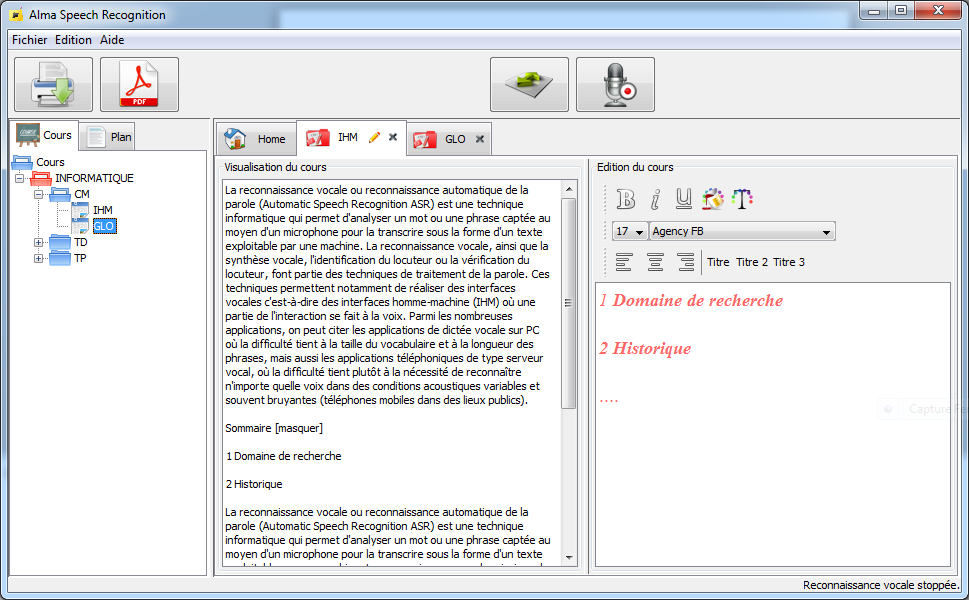
\includegraphics[scale=0.6]{./images/workPanel.png}
 % homePanel.png: 0x0 pixel, -2147483648dpi, 0.00x0.00 cm, bb=
 \caption{IHM - Panneau de travail}
 \label{fig:workPanel}
\end{figure}



